\documentclass[../main]{subfiles}

\questiontrue
\solutiontrue

\begin{document}
    \ifquestion
    
    \section{Orbital Sniper}
	
	Ramanu Jan discovers that someone has attempted to enter the airspace of his planet and is now trying to escape. At a certain moment, the invader stops at a distance $d$ from the planet to refuel their ship. Ramanu, being very merciful, only wishes to destroy the invader's ship with his super-powerful laser; however, he is prevented from taking a direct shot (in a straight line). Fortunately, he has an ace up his sleeve: a satellite in the shape of a 100\% mirrored plate that orbits the planet in a stationary orbit. The operation will consist of sending the satellite into a specific elliptical orbit, after which Ramanu will shoot at the satellite, which must reflect the radiation towards the ship.

Note: The mirror’s axis will always be tangent to the orbit.

Disregarding radiation pressure effects and relativistic effects, answer the following:

\ut{a} What is the minimum $\Delta v$ required for the operation to succeed?

\ut{b} Considering that the laser can emit radiation with intensity $I_0$ and that the medium permeating this region of space has density $\rho$ and opacity as a function of light frequency given by $\kappa=\kappa_0f^3$, what is the necessary frequency range for the ship to successfully explode, given that light with intensity $\frac{I_0}{2}$ is required for the engines to detonate?
	
	\clearpage
    
    
    \fi
    %%%%%%%%%%%%%%%%%%%%%%%%%%%%%%%%%%%%%%%%%%%%%%%%%%%%%%%%%%%%%%%%%%%%%%%%%%%%%%%%%%%%%
    
    \ifsolution
    
    \section{Orbital Sniper}

	\ut{a} The mirror must always be aligned with its orbital velocity, so it is as if Ramanu were shooting at the ellipse of the orbit itself, and it reflects. By Poncelet's theorem for an ellipse, it is known that if a light ray originates from one focus of the mirrored conic from within, this ray will converge at the other focus. Thus, we want the enemy ship to be located at this secondary focus so that the rays originating from the planet reach it. Therefore, $d=2ae$, where "d" is the focal distance, "a" is the semi-major axis of the orbit, and "e" is the eccentricity of the orbit.

To find the minimum $\Delta v$, we must determine the vector difference between the velocities at the transfer point of the elliptical and circular orbits. For this, consider the diagram in Figure \ref{fig:repreelipse}:
	
	\begin{figure}[htpb]
	    \centering
	    

\tikzset{every picture/.style={line width=0.75pt}} %set default line width to 0.75pt        

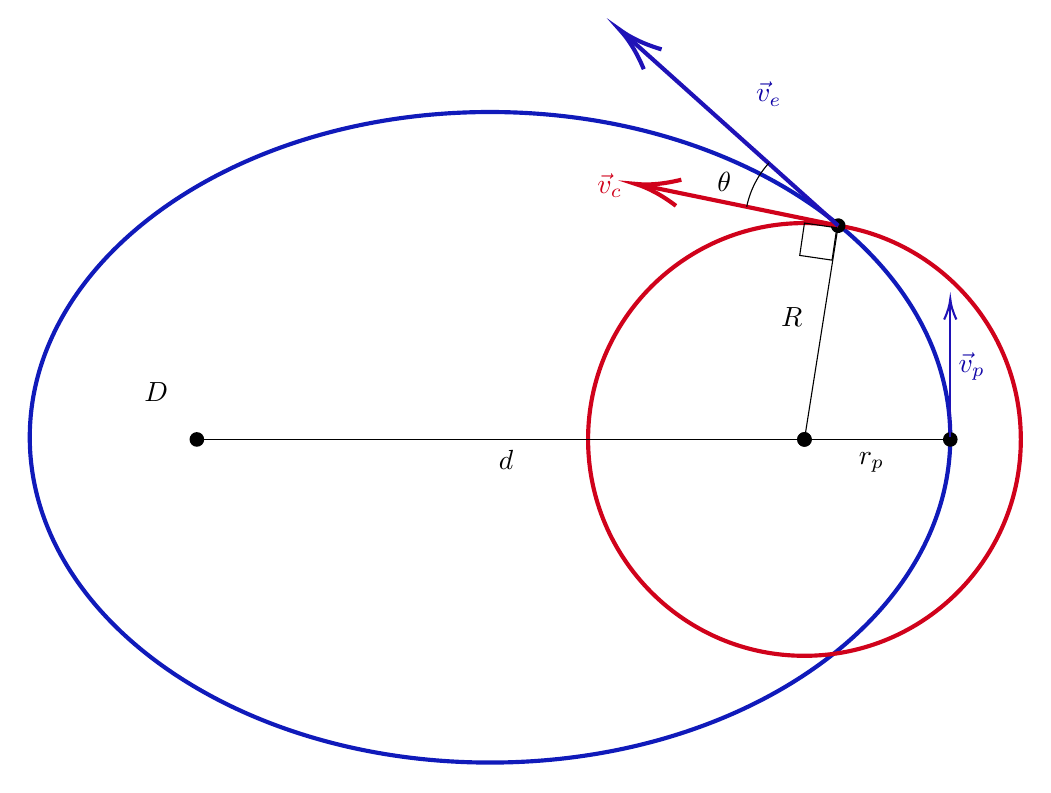
\begin{tikzpicture}[x=0.75pt,y=0.75pt,yscale=-1.5,xscale=1.5]
%uncomment if require: \path (0,542); %set diagram left start at 0, and has height of 542

%Shape: Ellipse [id:dp8979721006541848] 
\draw  [color={rgb, 255:red, 16; green, 26; blue, 186 }  ,draw opacity=1 ][line width=1.5]  (240,165.82) .. controls (240,108.12) and (306.19,61.34) .. (387.83,61.34) .. controls (469.48,61.34) and (535.67,108.12) .. (535.67,165.82) .. controls (535.67,223.52) and (469.48,270.3) .. (387.83,270.3) .. controls (306.19,270.3) and (240,223.52) .. (240,165.82) -- cycle ;
%Shape: Circle [id:dp31129963478340117] 
\draw  [color={rgb, 255:red, 208; green, 2; blue, 27 }  ,draw opacity=1 ][line width=1.5]  (419.33,166.51) .. controls (419.33,128.13) and (450.45,97.01) .. (488.83,97.01) .. controls (527.22,97.01) and (558.33,128.13) .. (558.33,166.51) .. controls (558.33,204.89) and (527.22,236.01) .. (488.83,236.01) .. controls (450.45,236.01) and (419.33,204.89) .. (419.33,166.51) -- cycle ;
%Straight Lines [id:da46140257439059673] 
\draw    (488.83,166.51) -- (293.67,166.51) ;
\draw [shift={(293.67,166.51)}, rotate = 180] [color={rgb, 255:red, 0; green, 0; blue, 0 }  ][fill={rgb, 255:red, 0; green, 0; blue, 0 }  ][line width=0.75]      (0, 0) circle [x radius= 2.01, y radius= 2.01]   ;
\draw [shift={(488.83,166.51)}, rotate = 180] [color={rgb, 255:red, 0; green, 0; blue, 0 }  ][fill={rgb, 255:red, 0; green, 0; blue, 0 }  ][line width=0.75]      (0, 0) circle [x radius= 2.01, y radius= 2.01]   ;
%Straight Lines [id:da7608233858325442] 
\draw    (488.83,166.51) -- (499.67,97.84) ;
\draw [shift={(499.67,97.84)}, rotate = 278.96] [color={rgb, 255:red, 0; green, 0; blue, 0 }  ][fill={rgb, 255:red, 0; green, 0; blue, 0 }  ][line width=0.75]      (0, 0) circle [x radius= 2.01, y radius= 2.01]   ;
%Straight Lines [id:da5987369599518098] 
\draw [color={rgb, 255:red, 208; green, 2; blue, 27 }  ,draw opacity=1 ][line width=1.5]    (499.67,97.84) -- (437.44,85.03) ;
\draw [shift={(434.5,84.42)}, rotate = 11.63] [color={rgb, 255:red, 208; green, 2; blue, 27 }  ,draw opacity=1 ][line width=1.5]    (14.21,-4.28) .. controls (9.04,-1.82) and (4.3,-0.39) .. (0,0) .. controls (4.3,0.39) and (9.04,1.82) .. (14.21,4.28)   ;
%Straight Lines [id:da304235614337492] 
\draw [color={rgb, 255:red, 31; green, 18; blue, 183 }  ,draw opacity=1 ][line width=1.5]    (499.67,97.84) -- (431.73,36.92) ;
\draw [shift={(429.5,34.92)}, rotate = 41.88] [color={rgb, 255:red, 31; green, 18; blue, 183 }  ,draw opacity=1 ][line width=1.5]    (14.21,-4.28) .. controls (9.04,-1.82) and (4.3,-0.39) .. (0,0) .. controls (4.3,0.39) and (9.04,1.82) .. (14.21,4.28)   ;
%Shape: Arc [id:dp11993801248437741] 
\draw  [draw opacity=0] (470.28,91.75) .. controls (471.38,86.41) and (473.91,81.59) .. (477.44,77.69) -- (499.67,97.84) -- cycle ; \draw   (470.28,91.75) .. controls (471.38,86.41) and (473.91,81.59) .. (477.44,77.69) ;  
%Shape: Square [id:dp709957464895024] 
\draw   (488.83,97.01) -- (499.22,98.53) -- (497.7,108.92) -- (487.31,107.4) -- cycle ;
%Straight Lines [id:da6564698637188566] 
\draw    (535.67,166.51) -- (488.83,166.51) ;
\draw [shift={(488.83,166.51)}, rotate = 180] [color={rgb, 255:red, 0; green, 0; blue, 0 }  ][fill={rgb, 255:red, 0; green, 0; blue, 0 }  ][line width=0.75]      (0, 0) circle [x radius= 2.01, y radius= 2.01]   ;
\draw [shift={(535.67,166.51)}, rotate = 180] [color={rgb, 255:red, 0; green, 0; blue, 0 }  ][fill={rgb, 255:red, 0; green, 0; blue, 0 }  ][line width=0.75]      (0, 0) circle [x radius= 2.01, y radius= 2.01]   ;
%Straight Lines [id:da10707508820939982] 
\draw [color={rgb, 255:red, 31; green, 18; blue, 183 }  ,draw opacity=1 ][line width=0.75]    (535.67,165.82) -- (535.67,123.42) ;
\draw [shift={(535.67,121.42)}, rotate = 90] [color={rgb, 255:red, 31; green, 18; blue, 183 }  ,draw opacity=1 ][line width=0.75]    (6.56,-1.97) .. controls (4.17,-0.84) and (1.99,-0.18) .. (0,0) .. controls (1.99,0.18) and (4.17,0.84) .. (6.56,1.97)   ;

% Text Node
\draw (276,147.41) node [anchor=north west][inner sep=0.75pt]    {$D$};
% Text Node
\draw (480.5,123.4) node [anchor=north west][inner sep=0.75pt]    {$R$};
% Text Node
\draw (460,80) node [anchor=north west][inner sep=0.75pt]    {$\theta $};
% Text Node
\draw (421.5,80.4) node [anchor=north west][inner sep=0.75pt]  [color={rgb, 255:red, 208; green, 2; blue, 27 }  ,opacity=1 ]  {$\vec{v}_{c}$};
% Text Node
\draw (472.5,50.9) node [anchor=north west][inner sep=0.75pt]  [color={rgb, 255:red, 16; green, 4; blue, 167 }  ,opacity=1 ]  {$\vec{v}_{e}$};
% Text Node
\draw (389.83,169.22) node [anchor=north west][inner sep=0.75pt]    {$d$};
% Text Node
\draw (505.5,170) node [anchor=north west][inner sep=0.75pt]    {$r_{p}$};
% Text Node
\draw (537.5,137.9) node [anchor=north west][inner sep=0.75pt]  [color={rgb, 255:red, 16; green, 4; blue, 167 }  ,opacity=1 ]  {$\vec{v}_{p}$};


\end{tikzpicture}
	    \caption{Representation of orbital transfer to elliptical orbit}
	    \label{fig:repreelipse}
	\end{figure}


By the velocity equation, we have:  
\[
|\vec{v_e}|=\sqrt{GM\left(\frac{2}{R}-\frac{1}{a}\right)}
\]

\[
|\vec{v_c}|=\sqrt{\frac{GM}{R}}
\]  

And by the law of cosines:  

\[
\Delta \vec{v}^2=v_e^2+v_c^2-2v_ev_c\cos{\theta}
\]  

For the calculation of $\cos{(\theta)}$, we use the law of angular momentum conservation for the elliptical orbit, as shown in the figure:  

\[
v_eR\sin{(\alpha)}=v_pr_p
\]  

Substituting the velocity at perihelion ($r=a(1-e)$) and the fact that $\alpha=90^o+\theta$, which implies $\sin{(\alpha)}=\cos{(\theta)}$:  

\[
\cos{(\theta)}=\frac{\sqrt{GMa(1-e^2)}}{v_eR}
\]  

\[
\therefore \Delta \vec{v}^2=v_e^2+v_c^2-2v_c\frac{\sqrt{GMa(1-e^2)}}{R}
\]  

Substituting the velocities:  

\[
\Delta \vec{v}^2=GM\left(\frac{2}{R}-\frac{1}{a}\right)+\frac{GM}{R}-2\sqrt{\frac{GM}{R}}\frac{\sqrt{GMa(1-e^2)}}{R}
\] 

Substituting $e=\frac{d}{2a}$, we obtain:

\[
\Delta \vec{v}^2=GM\left(\frac{3}{R}-\frac{1}{a}-\sqrt{\frac{(4a^2-d^2)}{aR^3}}\right)
\]  

Existence conditions are:  

\[
4a^2 > d^2 \Rightarrow a > \frac{d}{2}
\]  

And for the intersection between the ellipse and the circle (transfer point):  

\[
a(1-e) \le R \Rightarrow a\left(1-\frac{d}{2a}\right) \le R \Rightarrow a \le R+\frac{d}{2}
\]  

Finally:  

\[
\frac{d}{2} < a \le R + \frac{d}{2}
\]  

Now, analyze the following relation:  

\[
GM\left(\frac{3}{R}-\frac{1}{a}\right) - \Delta \vec{v}^2 = GM\sqrt{\frac{4a^2-d^2}{aR^3}}
\] 

Make the following substitution: $x = \dfrac{a}{d}$. Thus, the function inside the square root becomes: $\dfrac{d}{R^3}\left(4x-\frac{1}{x}\right)$. Note that $4x-\dfrac{1}{x}$ is increasing $\forall x > 0$, therefore:  

\[
\forall a_2 > a_1 \implies x_2 > x_1 \implies GM\sqrt{\frac{4a_2^2-d^2}{a_2R^3}} > GM\sqrt{\frac{4a_1^2-d^2}{a_1R^3}}
\]  

\[
\implies GM\left(\frac{3}{R}-\frac{1}{a_2}\right) - \Delta \vec{v}^2_2 > GM\left(\frac{3}{R}-\frac{1}{a_1}\right) - \Delta \vec{v}^2_1
\] 

\[
\therefore \Delta \vec{v}^2_1 - \Delta \vec{v}^2_2 > GM\left(\frac{1}{a_2}-\frac{1}{a_1}\right) > 0
\]  

Thus, we find that $\forall a_2 > a_1 \implies |\Delta \vec{v}_2| < |\Delta \vec{v}_1|$. Therefore, to choose the smallest possible velocity variation, we must select the largest possible value of $a$. That is, we will choose $a$ in the extreme case of $a=R+\frac{d}{2}$, when the perihelion of the elliptical orbit meets the circumference.  

In this case:  
\[
\Delta v^2=GM\left(\frac{3}{R}-\frac{2}{2R+d}-\sqrt{\frac{2((2R+d)^2-d^2)}{(2R+d)R^3}}\right)
\] 

\[
\Delta v=\sqrt{GM\frac{4R+3d-2\sqrt{4R^2+6Rd+2d^2}}{(2R+d)R}}
\]  

\ut{b} The effect of the medium's opacity will cause an exponential decrease in the intensity of the radiation as a function of the distance traveled, as follows:  

\[
I(r)=I_0e^{-\kappa \rho r}
\]  

where $r$ is the distance traveled by the light ray, which will be equal to $2a$ since, by definition, in an ellipse, the sum of the distances from a point to the foci is equal to the major axis. Since we want $I(r) \ge I_0/2$:  

\[
I(r)=I_0e^{-2 \kappa \rho a} \ge \frac{I_0}{2}
\]  

\[
I_0e^{-2 \kappa \rho a} \ge I_0e^{-\ln{(2)}}
\]  

\[
\therefore - 2 \kappa \rho a \ge -\ln{(2)} \Rightarrow 2 \rho \kappa a \le \ln{(2)}
\]  

Finally, since $\kappa = \kappa_0f^3$: 

\[
0 < f \le \sqrt[3]{\frac{\ln{(2)}}{\kappa_0 \rho (2R+d)\rho}}
\]

	\clearpage
    
    
    \fi
\end{document}
